\section{Planning}
\begin{justify}
    The following section will contain the Planning Phase of Software Development Life Cycle of Student Talent Development Center: Design and Implementation of Scheduling and Resources Management Web Application System.\\
\end{justify}

\subsection{Stakeholder Identification}
\begin{justify}
    The stakeholders of this system will include the users of the system which are the followings:
    \begin{itemize}[itemsep=0.1ex]
        \item Admin (STDC’s Administration/Staff).
        \item Student (Tutees).
        \item Tutors\\
    \end{itemize}
\end{justify}

\subsection{Activity Identification}
\begin{justify}
    The followings are the activities of each phase identified during which the development of the system should go through successfully and complete by the end of the project in order to deliver a complete system.\\
    \begin{itemize}[itemsep=-0.4cm]
        \item Planning \vspace{-0.3cm}
            \begin{itemize}[itemsep=-0.3cm]
                \item Identify Stakeholders.
                \item Identify Activities.
                \item Identify Task Duration.
                \item Produce Work Breakdown Structure.
                \item Identify Critical Path.
                \item Conduct Risk Analysis.
            \end{itemize}
        \item Analysis \vspace{-0.35cm}
            \begin{itemize}[itemsep=-0.3cm]
                \item Requirement Elicitation (gathering)
                \item Requirement Specification and Prioritization \vspace{-0.3cm}
                    \begin{itemize}[itemsep=-0.3cm]
                        \item Produce Use-Cases.
                        \item Produce Activity Model.
                    \end{itemize}
                \item Requirement Validation.
            \end{itemize}
        \item Design \vspace{-0.35cm}
            \begin{itemize}[itemsep=-0.3cm]
                \item Architectural Design
                \item Program Design. \vspace{-0.3cm}
                    \begin{itemize}[itemsep=-0.3cm]
                        \item Class Model.
                        \item Sequence Model.
                    \end{itemize}
                \item Interface Design
                \item Database Design \vspace{-0.3cm}
                    \begin{itemize}[itemsep=-0.3cm]
                        \item Produce EARD.
                    \end{itemize}
            \end{itemize}
        \item Implementation \vspace{-0.35cm}
            \begin{itemize}[itemsep=-0.3cm]
                \item Backend Development.
                \item Frontend Development.
            \end{itemize}
        \item Testing \vspace{-0.35cm}
            \begin{itemize}[itemsep=-0.3cm]
                \item Automated Testing
                \item Manual Testing \\
            \end{itemize}
    \end{itemize}
\end{justify}

\subsection{Task Duration Identification}
\begin{justify}
The following duration are presumed duration needed to finish each task. Each of the specified numbers are in days.
\end{justify}

\renewcommand{\arraystretch}{1.5}
\begin{table}[H]
\centering
\caption{Activities' duration}
\begin{tabular}{|p{9.0cm}|p{5.5cm}|} 
\hline
\rowcolor[rgb]{0.122,0.22,0.392} \textbf{\textcolor{white}{Activity}} & \textbf{\textcolor{white}{Duration (Days)}}  \\ 
\hline
Identify Stakeholders                                                 & 1                                            \\ 
\hline
Identify Activities                                                   & 1                                            \\ 
\hline
Identify Task Duration                                                & 1                                            \\ 
\hline
Produce WBS                                                           & 1                                            \\ 
\hline
Identify Critical Path                                                & 1                                            \\ 
\hline
Conduct Risk Analysis                                                 & 1                                            \\ 
\hline
Requirement Elicitation                                               & 3                                            \\ 
\hline
Requirement Specification                                             & 6                                            \\ 
\hline
Requirement Validation                                                & 3                                            \\ 
\hline
Architectural Design                                                  & 1                                            \\ 
\hline
Program Design                                                        & 10                                           \\ 
\hline
Interface Design                                                      & 7                                            \\ 
\hline
Database Design                                                       & 2                                            \\ 
\hline
Backend Development                                                   & 28                                           \\ 
\hline
Frontend Development                                                  & 28                                           \\ 
\hline
Automated Testing                                                     & 21                                           \\ 
\hline
Manual Testing                                                     & 32                                           \\
\hline
\end{tabular}
\end{table}

\subsection{Work Breakdown Structure}
\begin{justify}
The following tree shows the Work Breakdown Structure of the specified tasks above.
\end{justify}

\begin{figure}[H]
    \centerline{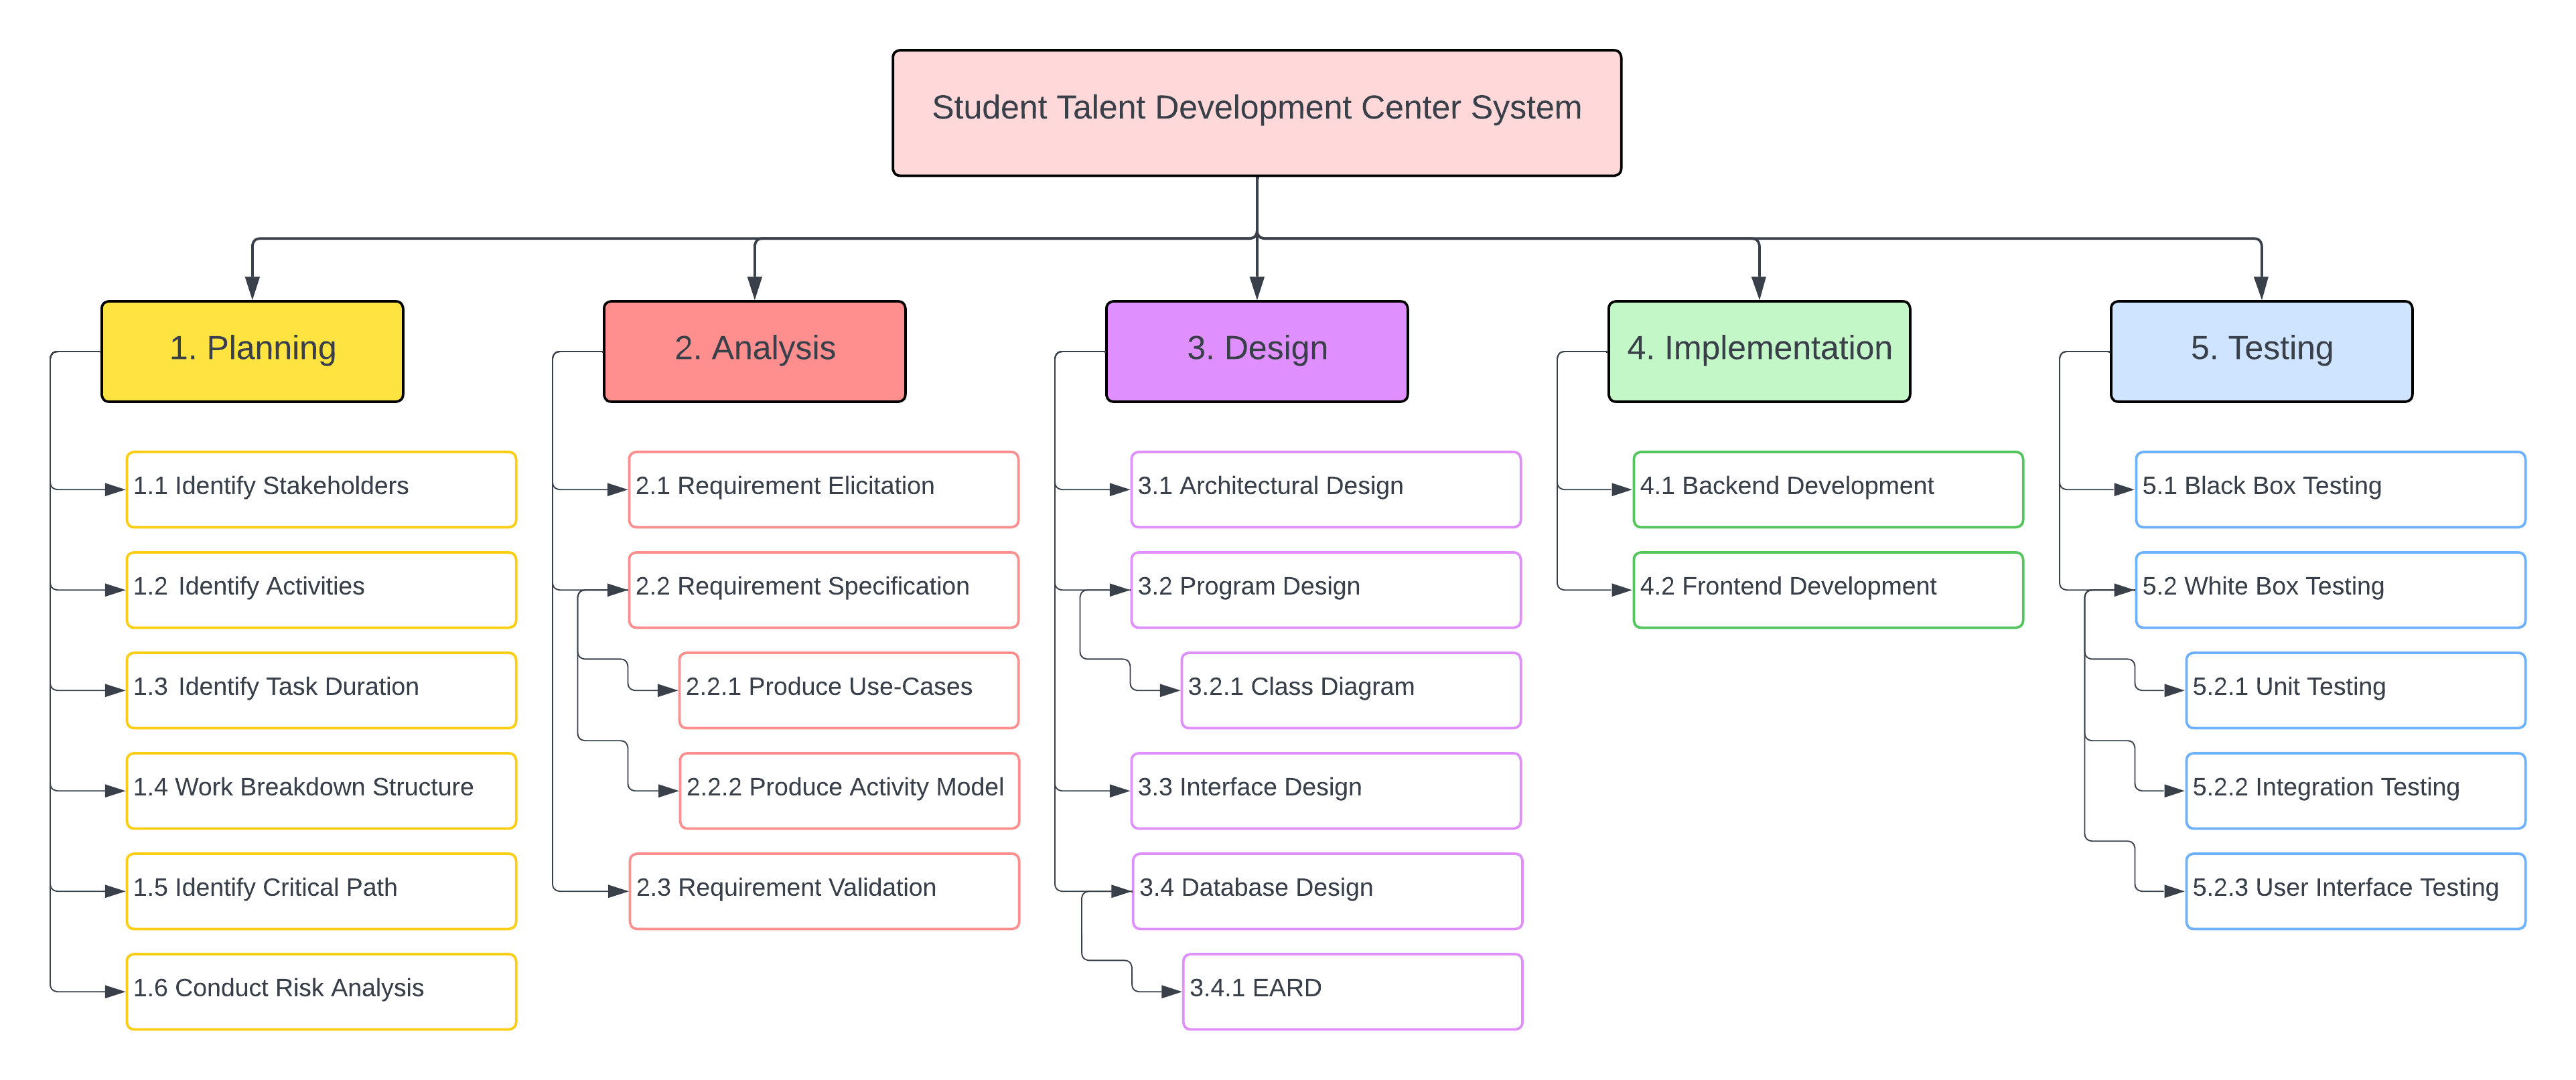
\includegraphics[width=150mm,scale=1]{figures/analysis_and_design/planning/WBS V2.png}}
    \caption{Work breakdown structure}
    \label{WBS}
\end{figure}


\subsection{Identify Critical Path}
\begin{justify}
The following is the finding of the critical path.
\end{justify}

\renewcommand{\arraystretch}{0.95}
\begin{table}[H]
\centering
\caption{Activity dependency table}
\begin{tabular}{|p{4cm}|p{5.83cm}|p{4cm}|} 
\hline
\rowcolor[rgb]{0.122,0.22,0.392} \textbf{\textcolor{white}{Activity}} & \textbf{\textcolor{white}{Predecessor}} & \textbf{\textcolor{white}{Duration (Days)}}  \\ 
\hline
{\cellcolor[rgb]{0.851,0.886,0.953}}1.1                               & 1.2                                     & 1                                            \\ 
\hline
{\cellcolor[rgb]{0.851,0.886,0.953}}1.2                               & -                                       & 1                                            \\ 
\hline
{\cellcolor[rgb]{0.851,0.886,0.953}}1.3                               & 1.2                                     & 1                                            \\ 
\hline
{\cellcolor[rgb]{0.851,0.886,0.953}}1.4                               & 1.1, 1.3                                & 1                                            \\ 
\hline
{\cellcolor[rgb]{0.851,0.886,0.953}}1.5                               & 1.4                                     & 1                                            \\ 
\hline
{\cellcolor[rgb]{0.851,0.886,0.953}}1.6                               & 1.5                                     & 1                                            \\ 
\hline
{\cellcolor[rgb]{0.851,0.886,0.953}}2.1                               & 1.6                                     & 3                                            \\ 
\hline
{\cellcolor[rgb]{0.851,0.886,0.953}}2.2                               & 2.1                                     & 6                                            \\ 
\hline
{\cellcolor[rgb]{0.851,0.886,0.953}}2.3                               & 2.2                                     & 3                                            \\ 
\hline
{\cellcolor[rgb]{0.851,0.886,0.953}}3.1                               & 2.3                                     & 1                                            \\ 
\hline
{\cellcolor[rgb]{0.851,0.886,0.953}}3.2                               & 3.1                                     & 10                                           \\ 
\hline
{\cellcolor[rgb]{0.851,0.886,0.953}}3.3                               & 3.2                                     & 7                                            \\ 
\hline
{\cellcolor[rgb]{0.851,0.886,0.953}}3.4                               & 3.2                                     & 2                                            \\ 
\hline
{\cellcolor[rgb]{0.851,0.886,0.953}}4.1                               & 3.3, 3.4                                & 28                                           \\ 
\hline
{\cellcolor[rgb]{0.851,0.886,0.953}}4.2                               & 4.1                                     & 28                                           \\ 
\hline
{\cellcolor[rgb]{0.851,0.886,0.953}}5.1                               & 2.1                                     & 21                                           \\ 
\hline
{\cellcolor[rgb]{0.851,0.886,0.953}}5.2                               & 5.1                                     & 32                                           \\
\hline
\end{tabular}
\end{table}

\begin{figure}[H]
    \centerline{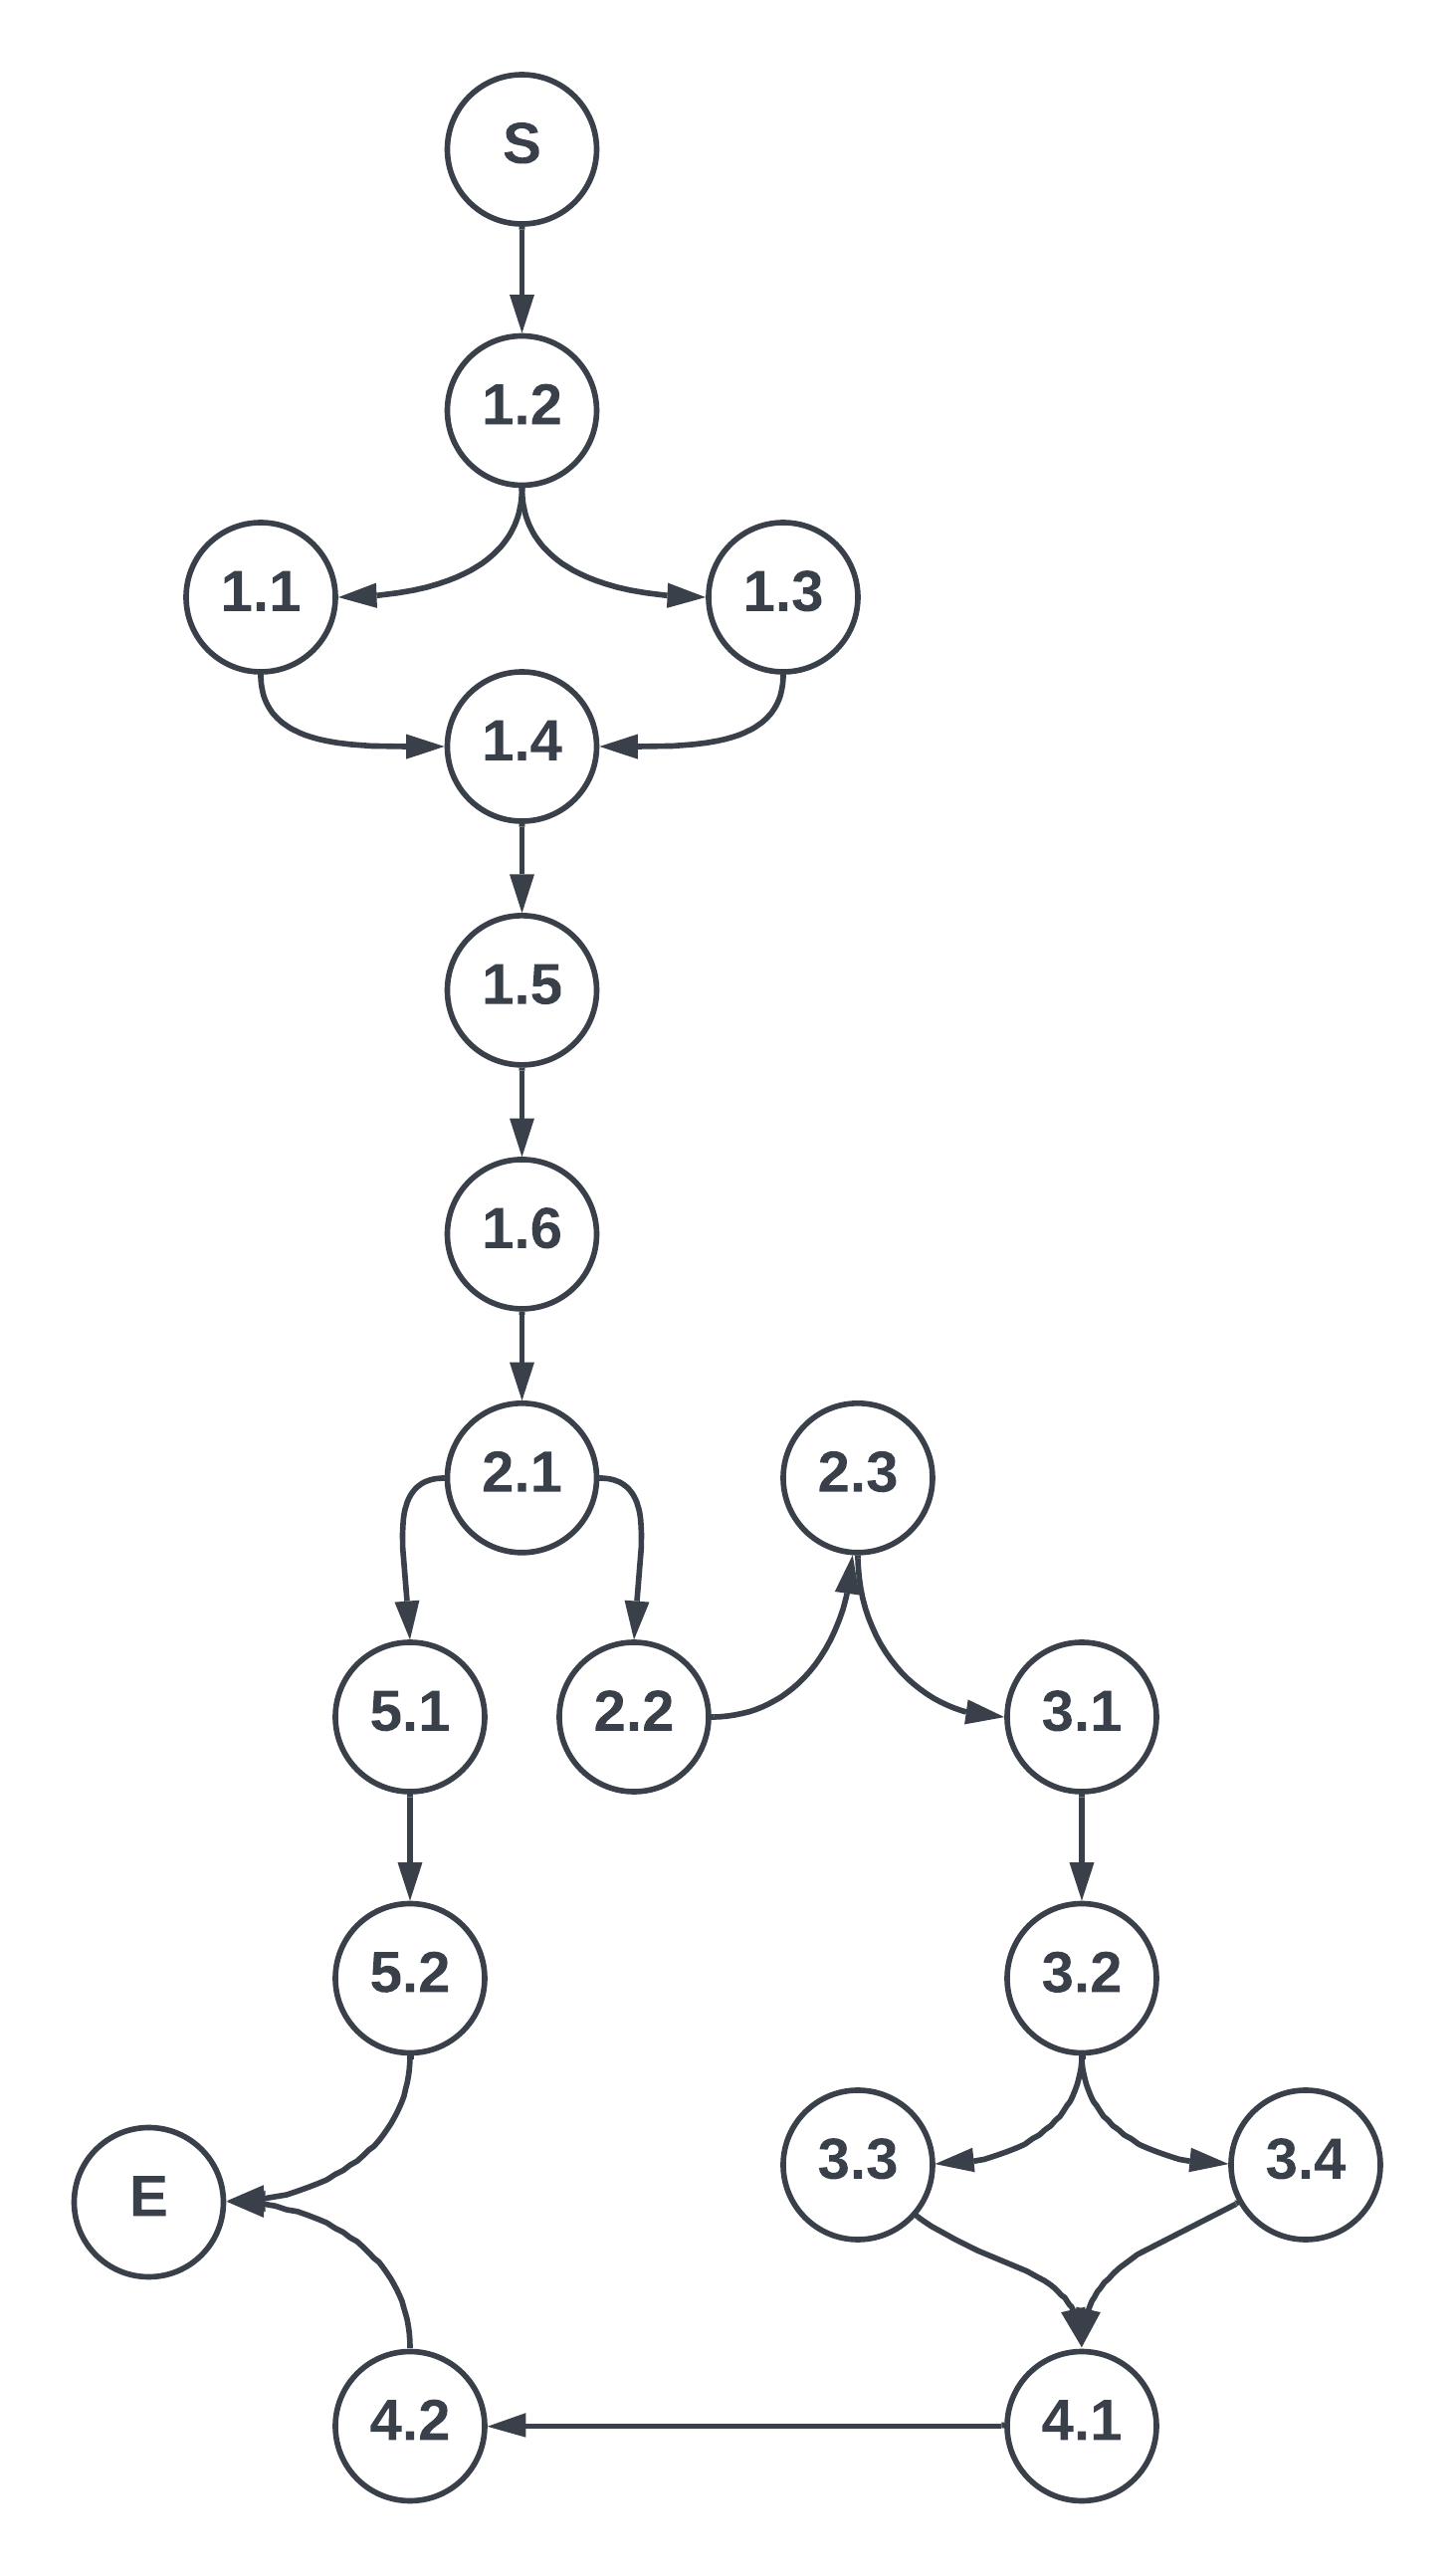
\includegraphics[width=130mm,scale=1]{figures/analysis_and_design/planning/Newtwork Diagram V2.png}}
    \caption{Network diagram}
    \label{networkDiagram}
\end{figure}

\begin{figure}[H]
    \centerline{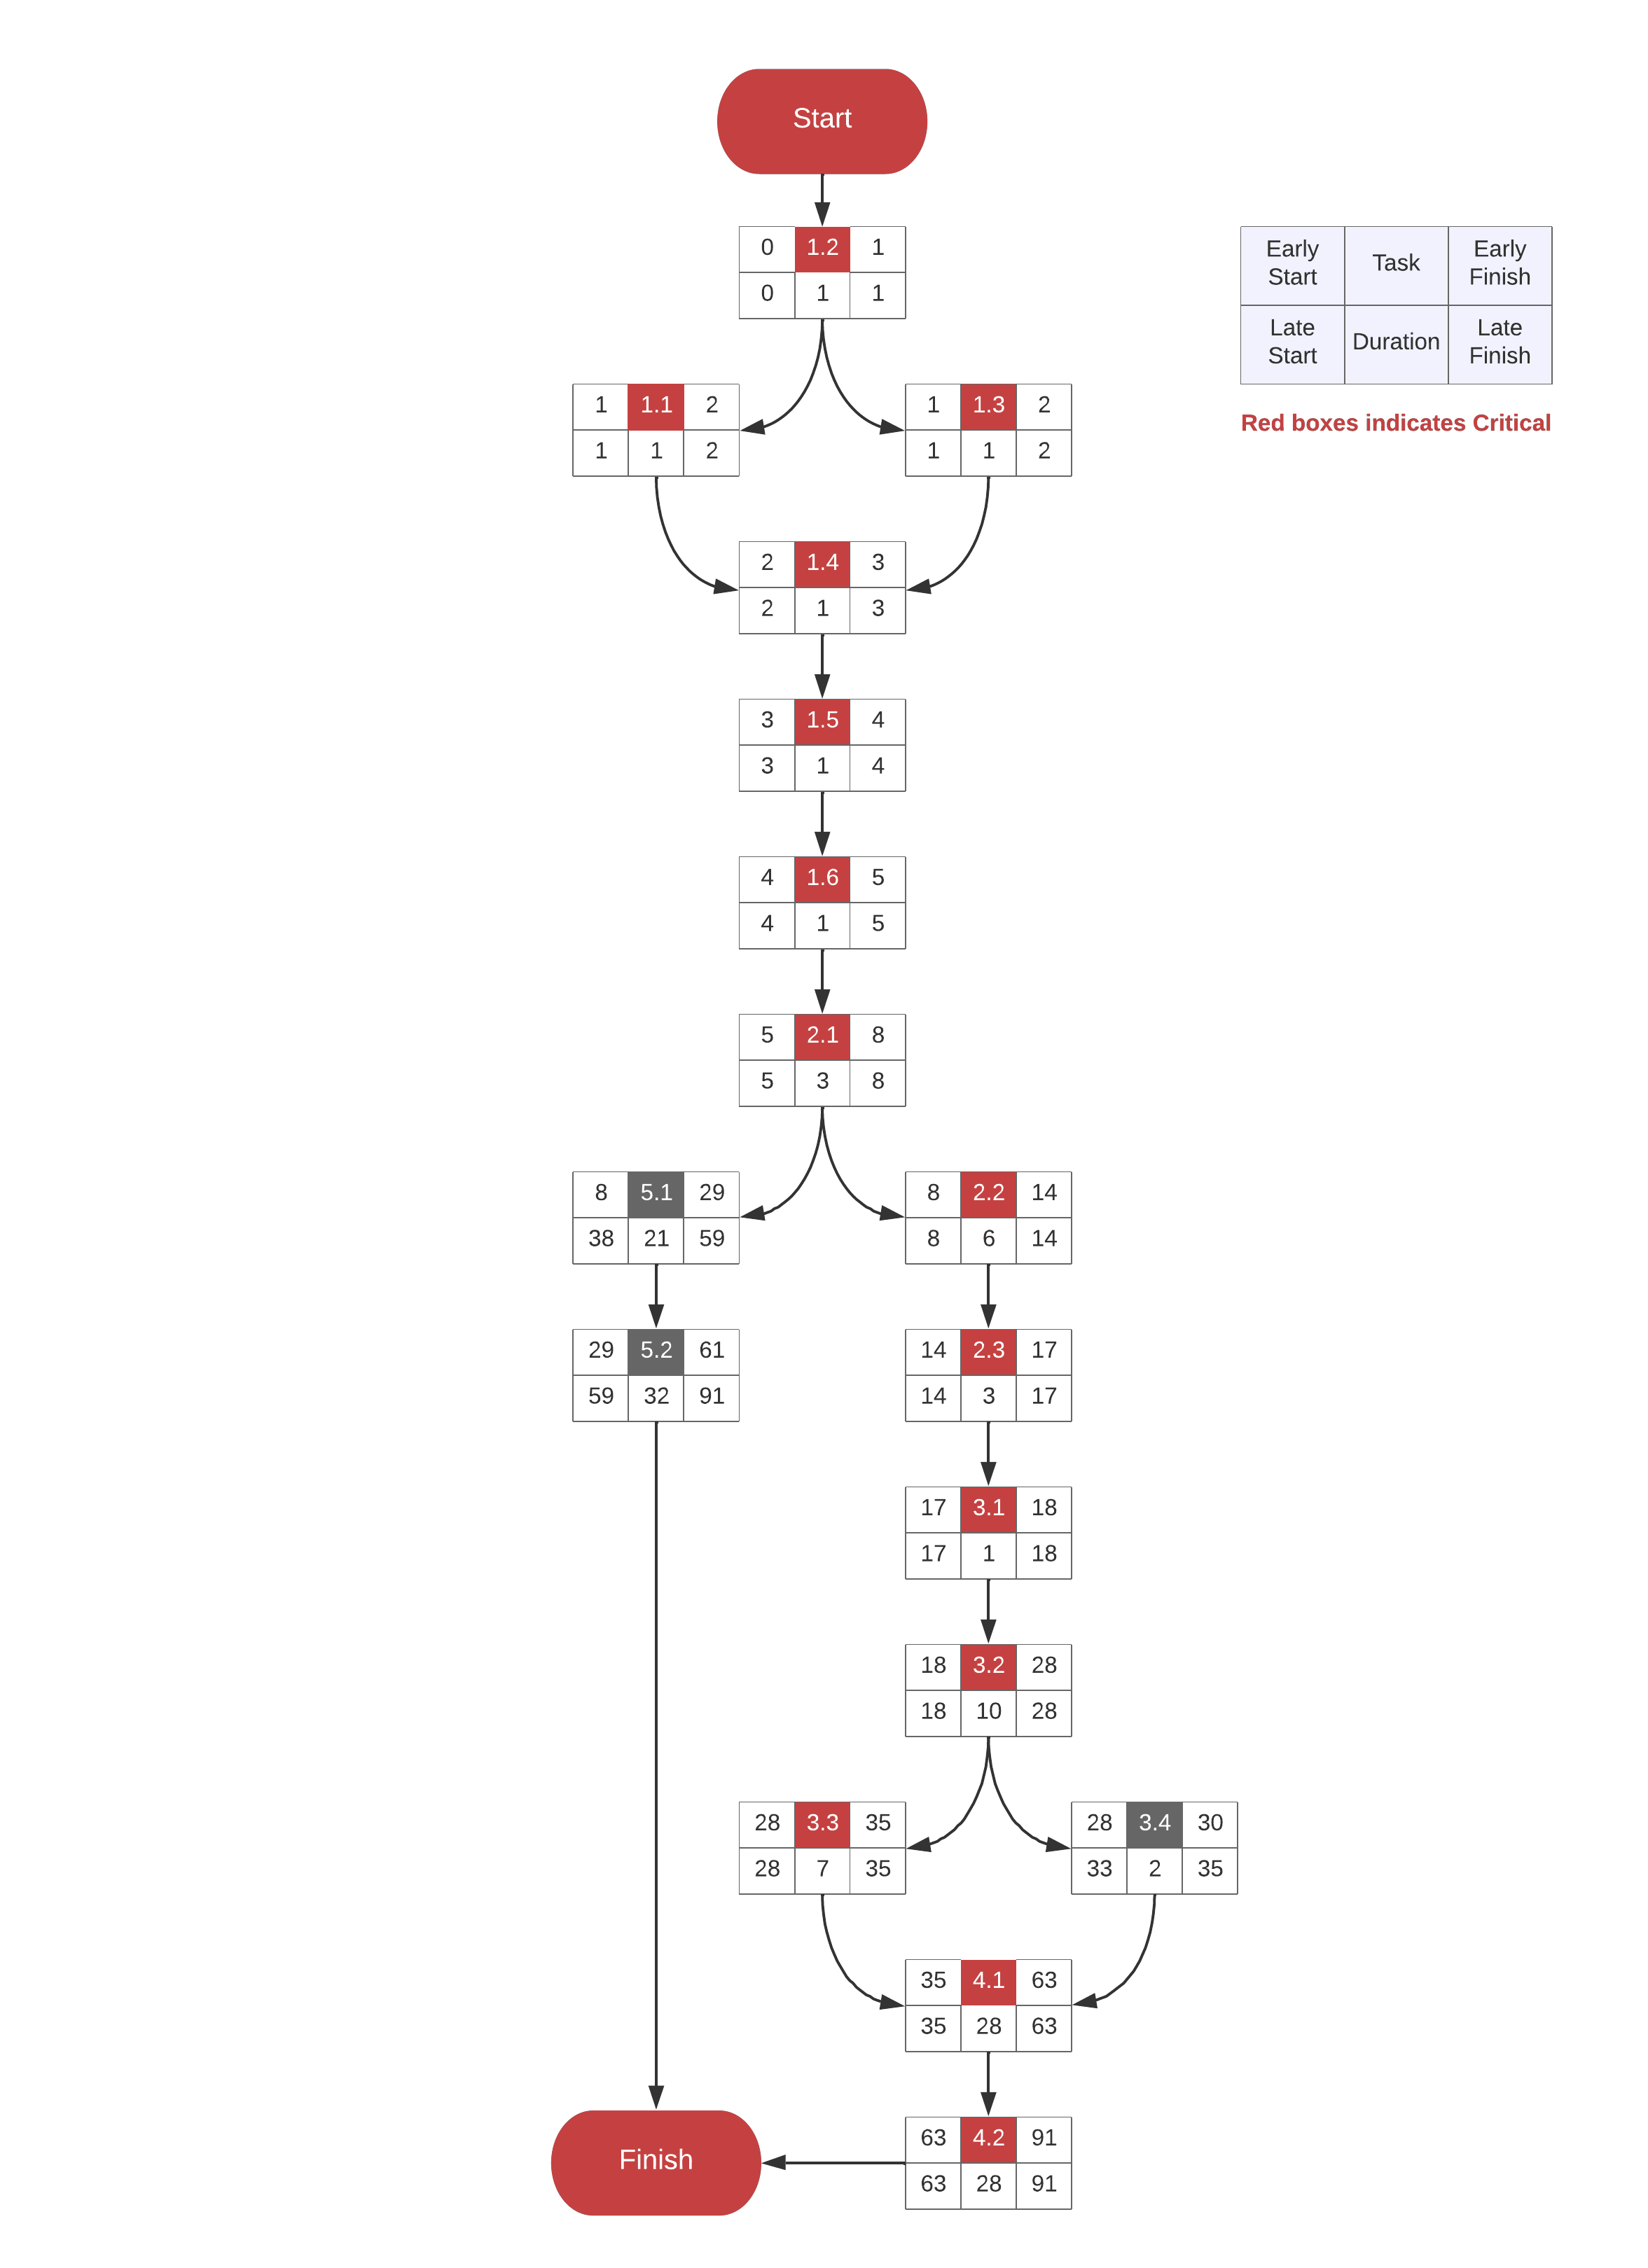
\includegraphics[width=170mm,scale=1]{figures/analysis_and_design/planning/Network diagram (PERT chart)- Cropped.png}}
    \caption{Critical path (pert chart)}
    \label{pertChart}
\end{figure}

\subsection{Risk Analysis}
\begin{justify}
The following is the risk assessment done through analysis of each risk, its likelihood, impact, mitigating strategies, and alternative solution in case of failure.

\begin{enumerate}
    \item Low Stakeholder Engagement
    \newendline A lack of stakeholder participation is one of the most frequent software development risks. This occurs due to a lack of communication between project stakeholders and developers, in this case me. In addition, sometimes stakeholders feel disregarded on the project's requirements, resulting in poor participation since they feel excluded/unaware of the project's status.

    \definecolor{vin}{RGB}{180,9,39}
    \newendline \textbf{\textcolor{vin}{Likelihood of the risk to happen:}} HIGH\\
    \textbf{\textcolor{vin}{Impact of the risk when it happens:}} HIGH

    \newendline Mitigating Strategy would be to have engaged in the project consistently by updating them regularly on project progress and encouraging them to be involved by confirming the requirements. Having regular meetings with them to keep the communication line with stakeholders can be another strategy to mitigate this risk.

    \newendline In case of failure, an alternative would be to confront stakeholders and remind them the purpose of the project and that their participation is to improve their lives. Listening to their problems and addressing them during more frequent meetings.\newendline

    %%%%%%%%%%%%%%%%%%%%%%%%%%%%%%%%%%%%%%
    \item Change of Staff or Management at Student Talent Development Center
    \newendline Although the likelihood of this occurring is low, the possibility still exists. UKH staff and management are constantly replaced. This raises concerns about having different personnel at STDC who may not cooperate or be involved in the project, as well as altering the center's business workflow. 

    \newendline \textbf{\textcolor{vin}{Likelihood of the risk to happen:}} LOW\\
    \textbf{\textcolor{vin}{Impact of the risk when it happens:}} MEDIUM

    \newendline Mitigating Strategy would be to immediately approach new staff/management upon their arrival at work. Explain to them the objective of the project and the significance of their participation, and have them alert me of any changes to the organization' workflow.

    \newendline In case of failure, an alternative would be to seek the assistance of former personnel or management in persuading new staff or management of the significance of the project and the need for their participation.\newendline

    %%%%%%%%%%%%%%%%%%%%%%%%%%%%%%%%%%%%%%
    \item Lack of Technical Skills
    \newendline In software development, technical risks are frequently a setback, something that is not instantly obvious but has severe negative implications. In an attempt to create a unique product, it is common to employ cutting-edge technologies, which might have a number of severe drawbacks and are hard to learn.

    \newendline \textbf{\textcolor{vin}{Likelihood of the risk to happen:}} HIGH\\
    \textbf{\textcolor{vin}{Impact of the risk when it happens:}} HIGH

    \newendline Mitigating Strategy would be to recognize my weaknesses and learn them before to the implementation phase. Sometimes it is difficult to anticipate these limitations, therefore when a risk develops during implementation, one response would be to seek assistance from colleagues and acknowledge their assistance.

    \newendline In case of failure, an alternative would be to postpone this functionality temporarily and concentrate on completing the other duties at hand, while conducting research to tackle the issue at hand. This is not always the best option, but it can save time and effort spent on a problem that cannot be solved at the moment.\newendline

    %%%%%%%%%%%%%%%%%%%%%%%%%%%%%%%%%%%%%%
    \item Incorrect Time Estimation
    \newendline A single day might result in substantial advantages or disadvantages in a project’s progress. There are a number of potential causes for time constraints, such as the wrong initial estimation and setting of the project's duration, a shortage of available technical knowledge, or an unanticipated and urgent new requirement.

    \newendline \textbf{\textcolor{vin}{Likelihood of the risk to happen:}} MEDIUM\\
    \textbf{\textcolor{vin}{Impact of the risk when it happens:}} MEDIUM

    \newendline Mitigating Strategy would be to have extra weeks available so that if a task is delayed, it would not affect the project's deadlines. An alternative would be to work more during a given week to prevent similar situations from occurring.

    \newendline In case of failure, an alternative would be to take a few days off work and concentrate solely on the project and its tasks. Catch up as quickly as possible.\newendline

    %%%%%%%%%%%%%%%%%%%%%%%%%%%%%%%%%%%%%%
    \item Resource Unavailability from UKH’s IT Department (Lack of Support)
    \newendline Although the possibilities of this happening are not high, nonetheless it is expected not to get support from IT Department of University of Kurdistan Hewlêr, since this project is not done through their supervision.

    \newendline \textbf{\textcolor{vin}{Likelihood of the risk to happen:}} LOW\\
    \textbf{\textcolor{vin}{Impact of the risk when it happens:}} LOW

    \newendline Mitigating Strategy would consist of constructing the required components and replicating the required data and services. This may take time, but it is the only viable option.

    \newendline In case of failure, an alternative would be to communicate with STDC administration in an effort to persuade them to assist and support by providing mock versions of their main services.\newendline

    
    %%%%%%%%%%%%%%%%%%%%%%%%%%%%%%%%%%%%%%
    \item Health Issues (Illness)
    \newendline Although health concerns can arise at any time for a variety of reasons and are hard to anticipate, it is not difficult to prevent known illnesses that could delay the project by days or weeks. This risk will disrupt the project's progress and cause delays that cannot be afforded. Considering the previous critical path, it is clear that the project must keep to its deadlines, with only a narrow window for delay.

    \newendline \textbf{\textcolor{vin}{Likelihood of the risk to happen:}} HIGH\\
    \textbf{\textcolor{vin}{Impact of the risk when it happens:}} MEDIUM

    \newendline Mitigating Strategy would be to follow the WHO's guidelines to prevent illness. Follow clean practices, use a mask, and avoid the public if it is not absolutely required. Testing frequently and early to prevent falling behind drastically.

    \newendline In the case of failure, an alternative would be to contact Registry and submit a mitigating circumstances form in order to extend the project's deadline. Although this is not the best solution, it is the only practical one.\newendline

     %%%%%%%%%%%%%%%%%%%%%%%%%%%%%%%%%%%%%%
    \item Unpredictable External Risks (e.g., Failing a Module)
    \newendline Unpredictable External Risks is another obstacle that might be confronted during project management. External risks in software development are not so uncommon, risks like introduction of new university laws, changes in the priorities of stakeholders, or even personal issues like failing a module could happen anytime.

    \newendline \textbf{\textcolor{vin}{Likelihood of the risk to happen:}} HIGH\\
    \textbf{\textcolor{vin}{Impact of the risk when it happens:}} LOW

    \newendline Mitigating Strategy would be to follow up with stakeholders on new priority changes, keep up to university works, and do not procrastinate on studying for this will be hard to mitigate.

    \newendline In the case of failure, an alternative would be to work in the weekends and holidays to focus on studies and university assignments.\newendline


     %%%%%%%%%%%%%%%%%%%%%%%%%%%%%%%%%%%%%%
    \item Making a lot of Assumptions
    \newendline When it comes to obscure requirements, it is easy for developers to develop an addiction to making a large number of assumptions. This results in a different product or a product that does not address the issue at hand. And often, starting from scratch is a burden because it is both time-consuming and requires a larger expenditure than allocated. Given that the time frame for this project is extremely tight and does not permit redoing a feature, it is essential that no assumptions be made regarding how things should function.\\

    \newendline \textbf{\textcolor{vin}{Likelihood of the risk to happen:}} HIGH\\
    \textbf{\textcolor{vin}{Impact of the risk when it happens:}} HIGH

    \newendline Mitigating Strategy would be to communicate with stakeholders more frequently, to take their ideas into consideration, and to clarify matters that are unclear.

    \newendline In the case of failure, an alternative would be taking advice from professors who have a good background in systems development and take their opinion on certain matters.\\

    \newendline \textbf{Risk Assessment Findings}

    \newendline The Student Talent Development Center project risk analysis was concluded by examining a variety of hazards across domains. This evaluation identified possible project roadblocks, assessed their likelihood and impact, and developed preventative actions and alternatives if the risk materialized.

    \newendline This risk assessment acknowledges that every endeavor has risks. The analysis focused on anticipating and mitigating these hazards. Risk management is continuous, nevertheless. As the project continues, the risk environment may change, requiring regular analytical updates. While we've tried to anticipate the biggest dangers, it's important to be flexible to handle the unexpected. To complete the project, these risks must be managed.
\end{enumerate}
\end{justify}

\clearpage


